\chapter{Low Data Complexity Power/EM 2}

We want to see what is power analysis all about and see a very simple power
analysis attack that we can actually perform. Then we will dive into AES and its
implementation.

All the things that we will see today are very optimistic and they assume that
we have really good measurements, very good understanding and very good luck,
but it's actually quite a little bit harder in practice.

\section{The New York Times, Take 2}
The hero for this article is Mister Kocher. He discovered something that can
attack smart cards with what's called power analysis. Probably it was discovered
before, but he has discovered it academically.

What did he do? He went to a conference and took people's smart cards and found
out their secret private keys. We saw last week that if we have to sign
something and we have the private key you can sign a thing that's not supposed
to be signed and steal money, this was a big deal.

The 1995 timing attack went to the front page of the New York Times and there
was a lot of discussion about the discovery. The 1998 result about power
analysis only goes to the bottom of page two in one of the supplements and
actually nobody has discussed about it a lot. 

Why didn't he get a lot of attention for this power analysis attack? Could be
because timing is one thing and power analysis is a little more complicated but
in the bottom line we can see all the secrets. To do a timing attack you need a
stopwatch, while to power analysis attack you need more sophisticated equipment.

\section{Power Analysis Attacks}
What we need to make timing attack? We just need to be able to send request and
gets responses to measured how much it took, while the target can be at the
other side of the internet (can Amazon Cloud very far away).

What we need to make Power analysis attack? We need to be physically. How do we
connect to the device? We need to cut the power supply and connect to it
diractly to measure the power consumption. This is a very invasive attack, we
need to be very very close. in 1995 let's assume that it's true. so if we go to
the system architect:” listen there is an a power analysis attack that's can
completely compromised the device. Attacker needs to come to the device end cuts
the power supply….” by the time you already lost the system architect because
this is not practical. The threat model has to make sense.
 
nevertheless, the threat model does make sense in a lot of scenarios and we
discovered that thing that we was not supposed existing these power analysis and
side Channel attack. today we can attack this device and tomorrow we can attack
another device.

To learn about power analysis attack you can go and search in the library the
“Power Analysis Attacks” book.“Cryptanalytic attacks that allow extraction of
secret information from cryptographic devices by exploding their power
consumption characteristics”let's see what can we discover from this definition.
First, What we are attacking here? Cryptographic devices. what we are not
attacking? cryptographic algorithms. If I told you that I was able to break RSA
on my phone by doing power analysis did I break RSA? No we didn't break RSA, we
break the implementation of RSA. What else we are not attacking? The user is not
under attack, we are not doing any key logging or human engineering attack or
social engineering we are only attacking the device. What's the cryptographic
device? Some kind of crypto, signing or encrypting. What a secret information we
wants to extract? Probably we extract the key. And what's nice about the key?
That he has lots of bits. At the start you don't know anything about the key, If
you get half of the key you halfway, if you get the whole key You win. If I want
to make the device more secure what do I need to do to key? we make a longer
key.

This is very easy to say, but if I'm talking instead of secret information we
cracked from the device, like medical information, it's a little harder to
understand what we can do with half of it. How do we make the medical
information more secure? What it's actually means?

Let's take credit cards, the companies say that you are more secure with credit
card. Why do we think that we have a privacy with credit cards? We are giving
the credit card number and our name... Looks like we're giving everything, the
saying that we are actually have privacy, a lot of people have in the US have
the same name, but you also get a zip code. Every time you pay with the credit
card it generate a new credit card number automatically and doesn't have any
digits on him. It is very hard to talk about privacy if it's not a
cryptographic. What's left from the definition? we are exploiting the power
conceptions characteristic.

What are we not exploiting? We're not doing math and we are not doing something
that you can do by algorithms. It's important to know that exploiting the power
at conception characteristics does not have to be actually measuring the power.
We saw last week that we can actually measure the power consumption with other
methods. When Kotcher wrote his paper he announced three types of power
analysis. One of them called Simple power analysis, the other one called
differential power analysis. Let's see the simple power analysis today.

\section{Simple Power Analysis}

The simple power analysis means that I'm going to take the measurement of the
device, making one measurement or two. With that we are going to get the key
from those measurement. What's nice about this attack that it's very reasonable
attack model. We need to get the power consumption trace ( this is a vector
overtime of the power consumption of the device), and we need only one or two
traces. This is actually durable in a lot of scenarios even if I have the device
for a little time or even if someone is looking at me. We will see the setup
that can be used for simple analysis. 

When you go to a store in Europe, you can't give the credit card for the
cashier, they give you this terminale and then you need take your credit card
insert it and put the pin number. And what is going over here, there is
something like a cryptographic computer between your card and terminal. Let's
assume that we want to attack the card, and it is in my possession. This model
is very permissive to me and I can do whatever I want, I can do a lot of
transactions I can do radiat, I can twist it and even melt it. so attacking the
card is very easy.


But if I don't wants to attack the card? I want to attack the terminal using
power analysis. Maybe the terminal has an SSL private key which is used to
connect to the Central Center, and this can make a lot of damage and we can be
very rich.

We want to do a power analysis on the terminal. This is a nice setup, this is
something that looks like a credit card, but it has are wired connected to this
fpga and connect to a computer. I will be in a very cold country and I will take
this card out from the jacket to my palm. Insert this chip into the terminal,
while doing a power analysis on a this terminal. The idea is that I can do it
about 1 or two times, but not making it for a thousand times or melt it. I can
attack maybe this terminal or a gas station. The fact that we don't need a lot
of traces is actually good.

What are the disadvantages? The problem here is that when I look at this power
trace I need to be very very well prepared, and understand what's really going
on in the power trace. Because we get a vector with a hundred thousand points
and we need to understand where is the encryption starting? Where it is ending?
What it means that there is a lack of power here a little power there? We need
to have a very good understanding of the device processes. 

Not only that we need also to have a very good measurements, because I only have
one or two measurements. They're a lot of external Influence on the device,
there can be noise, may be related to the device may be related to the
environment, and if I have only one measurement I am going to get all of this
noise at once and cannot do anything to reduce it. Statistically I'am not going
to be able to get clean measurements to perform the attack.

Another problem is that I will need to work very hard to find the key. Let see
an example: Yossi did a power analysis measurements and he got a Trace and there
was a noise, he did his analysis and got the key. Now he want to check if this
is the right key. How can we check the key? Try to decrypt and encrypt the
private key. Is this the right key? no it's not :( .. Why? We have only one
Trace. Maybe there was noise? Maybe one measurement was wrong? How do we recover
from this? We can try a similar key and not there exact key, maybe to change you
on bit here or there. This search might be so intensive that we getting
basically the same effect like a Brute Force. This makes simple power analysis
are not very effective because of all of those reasons.

\section{Other Types of Power Attacks}

So in general in power analysis there are two classes:

\paragraph{Low data complexity attacks} where I get line trace or two traces (a
very small amount of traces). Then I do a lot of post-processing and think
really really hard and maybe do a reverse engineering before.

\paragraph{High data complexity attacks} I will talk to you about it next week.
These attacks require a lot of traces, maybe thousands or Millions traces, a
Terabyte of data.

\section{Tuning the power model}

 The first thing that you need to do for a simple power analysis attack is to
 understand what device you are attacking. We attack two general types of
 devices with simple power analysis, first is a microcontroller or a CPU and the
 other thing is ASIC. 
 
Microcontroller is basically a regular computer, it gets commands and runs it
one after another, if you want to write a new software for this computer you can
write it in C or Java, they're cheap and commonly used.

\begin{figure}[htp]
\hspace*{0in}
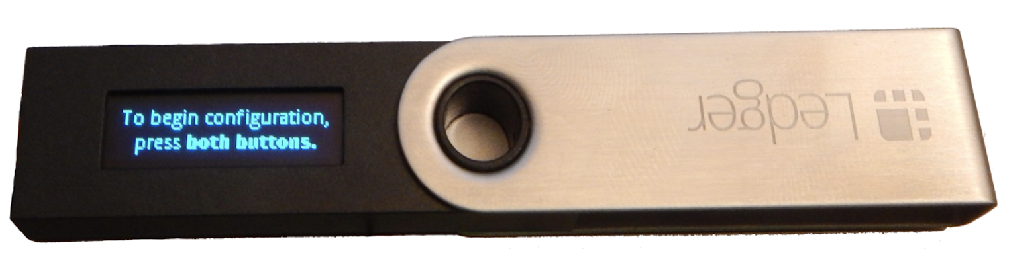
\includegraphics[scale=0.3]{images/Lecture_5/ledger.png}
\caption{Bitcoin Wallet}\label{fig:Bitcoin Wallet}
\end{figure}

This is a Bitcoin wallet. The Bitcoin is basically numbers and if someone steals
these numbers he steals your money, so you don't want these numbers to be on
your computers. These do all the calculation when you connect to the network, we
want it to be very secure because if someone steal the secret key he can take
all of your money.

\paragraph{}
Inside this device it has an orange Square and this is the microcontroller. Her
some storage and you can write some code for it.

The other kind of a device is called ASIC, this device is manufactured only for
a specific purpose. Let's say I want to have a sprinkler that starting the
morning and ends in the evening, I will use a programming language that called
HDL, once I compiled these software I am not getting an executable program that
I can run on a device. These chips can only do one thing, I can't programming
them and I can't upgrade them, if there is a bug I am in a big problem, but they
have only one purpose. The power consumption of this devices are going to be
smaller and sometimes they even be faster. Microcontrollers have programs that
runs one line after another, an ASIC can do a parallel operation. ASIC is very
cheap to manufacture, but there is a big wrap up before you produced this.

In this course we are going to talk only about microcontrollers, because we are
going to see them more often than ASICs. But you will know enough to open the
book attacking ASIC.


\begin{figure}[htp]
\hspace*{0in}
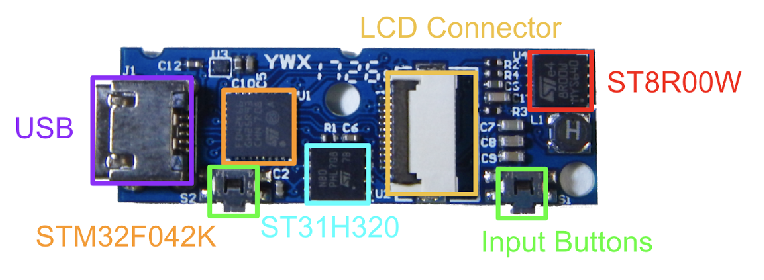
\includegraphics[scale=0.4]{images/Lecture_5/arduino.png}
\caption{Arduino}\label{fig:Arduino}
\end{figure}

So what is the line between microcontroller and an ASIC? On one of the student
table there is a chip that he will show us, this is a FPGA field programmable
this chip. If I want to identify a particular face I can program this ASIC to do
patterning for this face and doing it very very cheaply. I can do also audio
compression maybe I don't know what exactly I want to do but I know that I need
to do some kind of compression while I don't know exactly the algorithm by using
this ASIC. So you will find an ASIC if you have a piece of equipment 10000
pieces, maybe a router ,oscilloscope, submarine and things like that. Best to
make sure what is an Arduino? Microcontroller. 


\section{8-bit microcontroller}

This is an 8-bit microcontroller from the 80s, you see the center of this
microcontroller , this pair of trousers the red that named ALU, this is where
the magic happens, this piece of silicone can actually do logic like multiply,
add, shift or compare. 

\begin{figure}[htp]
\hspace*{0in}
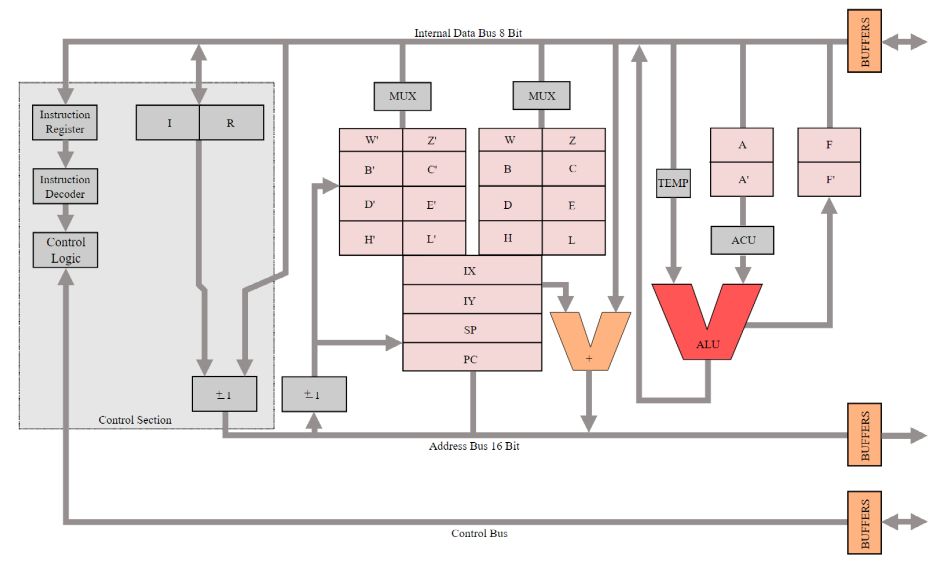
\includegraphics[scale=0.3]{images/Lecture_5/8bit-mc.png}
\caption{8-bit microcontroller}\label{fig:8-bit microcontroller}
\end{figure}


The entire process of life is to get a line of code which represent an
instruction, he has to understand what this instruction is trying to do. It can
be multiply, read or write. And then you get the operator you need to do from
the memory and fed it to the ALU. Then we'll get the next instruction and we'll
do it again and again. what's important for me to show you that there is two
long in lines from the top and the bottom they are called the buses. the top
called the data bus and the bottom call address bus. What is data bus mean? Any
sort of data you need to computation has to fetch from this bus. If something
come from the memory it going from this bus. If I want to write to external
input output, it also going on this bus. The width of this bus is 8 Bits and it
means all of the operation that this microcontroller do our eight bits.

On the bottom there is another big bus which is the address bus. If I want to
write to memory, I'm going to put their address in the address bus and then I'm
going to put the data in the data bus. I will set the control bus to write, and
then the memory which is somewhere else is it going to rise to this address. If
I want to do a read, I will put the address I want to read in the address bus,
and read in the control. What I will do in the data bus? I don't want to put
something in there because I want to read, this is actually important and I will
elaborate about it more later.

\section{Power Model for Microcontrollers}
What's interesting about microcontroller that there are in many cases the power
model don't have Hamming distance and actually have Hamming Weight. What does
that mean? That if I think that there are going to be a value going over the bus
I don't need to know what was the previous value on the bus, because it's going
to be exact humming weight for this value. 

When you have the best that is shared with several components the idea is that
all of the components that are not using the bus are going to set how to put
them, so all are ones, So if I want for example to read advice from memory the
CPU is going to set everything to one and then he is going to extract the memory
from the address, then the memory is going to lower all the relevant bits until
what sitting on the memory bus and the data bus what I wanted. 

Let's say I want the memory 4, at first I'm going to see on the data bus 0xFF,
then I will see 4 and then going to see agaoxin FF because the memory is
finished. what was the power-consumption here to go from FF to 4, how many beats
has to change? 7, and again it goes back to FF.

\section{Simple Power Analysis of RSA}
Let's see the power module this device under test, which does RSA decryption or
signing. While it's doing it we are getting the power measures. Why it is doing
an RSA decryption? Because it needs it. We can do it by sending encrypted emails
from the phone, so you really have to decrypt the message.

\begin{figure}[htp]
\centering
\hspace*{0in}
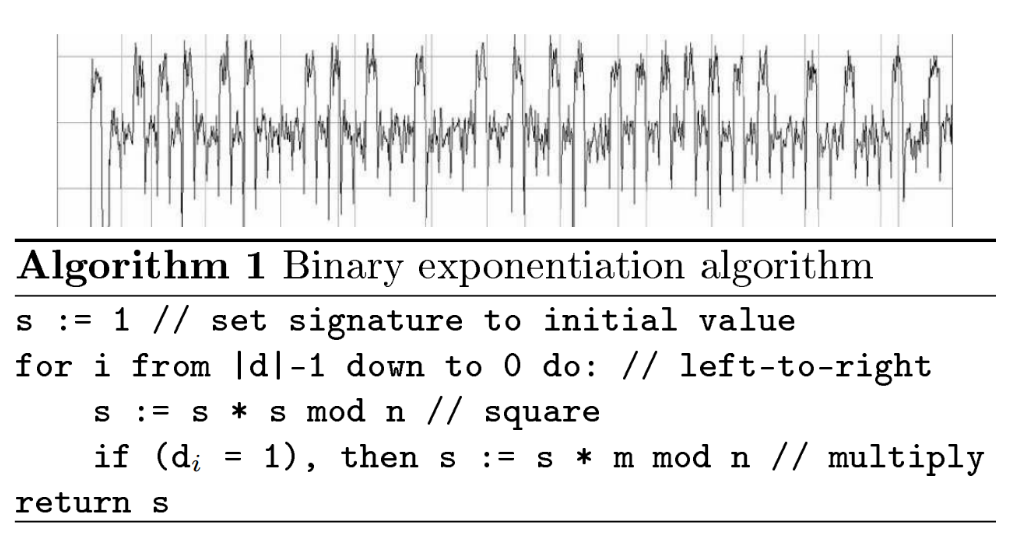
\includegraphics[scale=0.3]{images/Lecture_5/RSA-PA.png}
\caption{RSA Power Analysis}\label{fig:RSA Power Analysis}
\end{figure}

The axis are vector of power measurements, x is time, y are the power
consumption,(how did we measure the power consumption? i put a probe, measer the
voltege so on.. What is the private key? What is missing? You need to do some
reverse engineering first. If this is the only chance to get the key, I need to
tell you a little bit more about the device so you will understand what is going
on here. This device is microcontroller, it's doing RSA decryption using right
to left binary exponentiation using square and multiply. Is it helping you
finding the key? Yes. Let me show you the source code.

Binary exponentiation, it starts from the top most bit, off the secret and
privates decryption key, and then for each bit we do Square and multiply. If the
bit is zero we do Square, if this bit is one we do square and multiply. This
help you now finding the key, let's look at that Power Trace.

We see two types of things here, this little thing and the big thing. We have
some little thing, big thing, little thing, big thing, and then little little
little, and then big thing.

All we need to do is to be able tell about were is the square and were is
multiply, and then I can read the key, from top to bottom. So telling about
square and the multiply to get to the key is the general method. We see square
is take a little power and multiply more power.

What is square? square is multiply. So why is the power consumption of square
using multiply is different? this is a microcontroller and his bus width is 8
bit. He's doing a convolution between numbers, so it's multiply thousands of
time in frame. so why this is different? So what is consuming power, the ALU is
consumer power, the data bus and the address bus consuming power. In this case
the power consumption module of the address bus is hemming distance, because
it's not setting to 1 between accesses it's always containing what CPU is
writing. So did you and multiplication, you are going to see a lot of difference
values written into memory to the address bus because this microcontroller have
very small component ALU always fetching addresses from memory so ding s*s it's
fetching thousands of thousands of memory, but the address is fetching is very
similar to each other, because they are all s. les say s is 1k bits in memory
all the above are the same but the bathroom are different.But here we are doing
s time m, so it's fetching s and m, and you doing convolution. so the address
bus when it's doing S and M it's changing a lot, because he needs to do not only
the bottom bits but also the top bits.

\section{Simple Power Analysis of AES}

I am going to attack an 8 bit microcontroller. Let's look on the setup. This
microcontroller has a secret key, and it uses an AES encryption. We can ask him
to encrypt and decrypt, we send the command in the serial line.

\begin{figure}
\hspace*{0in}
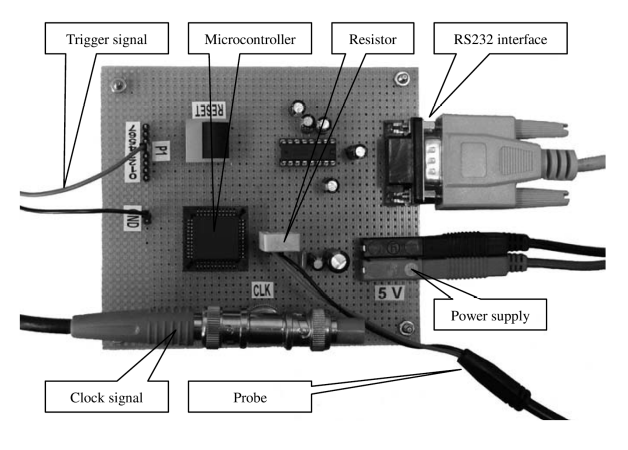
\includegraphics[scale=0.5]{images/Lecture_5/AES_setup.png}
\caption{AES Setup}\label{fig:AES Setup}
\end{figure}
 
While he's doing this operation it is going to consume different amount of power
and we would like to measure that. How do we going to measure them? We going to
connect to the microcontroller power supply. But were do we need to cut and
connect? The power is not going straight to the device it is going from this
white box (small resistor). How much power is going to go through the resistor?
Because he's small it's going to take very small power consumption. The voltage
drops across this device is going to be measured by this Probe, and I'm going to
measure the voltage over time. We know the voltage of the power supplies is 5
volt, so from this we can find out what is the current going through the
microcontroller and from the current we can find out what is the power
consumption. Do we need the code of the microcontroller? Yes. The only thing I
don't know is what? The secret, but I know everything else.
 
\section{Advanced Encryption Standard} 
 
What is the story about AES the encryption standard. 

In Death Valley Days encryption was in military standards it was considered like
a weapon you weren't supposed to have encryption, not by buy, export or sale.
but in the seventies the US government what is it might be a good idea to have
civilian encryption to protect civilian identities or health. they went to IBM
and ask them to write civilian encryption standard. IBM gave them an algorithm
called “Lucifer”, which was based on civilian Knowledge from the World War II,
the NSA I analyzed it and they say they don't actually like what you wrote and
change it. they changed the key change one of the internal tables and say this
was the standard. and the DES actually announced. the changes that NSA made was
making it difficult to implement it in software, and to make it Brute Force
about using the computing power that has the NSA but to protect it against some
kind of attack which was known to the NSA but not known in the Differential
cryptography ( not going to teach you).

The time passed and the computer got more and more powerful, there was something
called Deep cracking the electronic something, which was able to crack DES at
least. I'm not sure if they built it. This was too weak, so introduce something
called triple DES, it was twice as secure. Triple DES only used two keys, but
we're not going to study in this course. This wasn't so very efficient and it
was very slow. The US National standard unit, we want to create a new Cipher
which was at least as secure as Triple DES but much more efficient. Efficient on
software and hardware and slow computers. Anybody could submit candidates, the
winner of this competition was AES, which was a PhD work Raymond and Diamond.

It has some very good properties that we are going to talk about them.

\section{The Advanced Encryption Standard} 

How would you say AES is?, it is an operation which take 2 input, a kye and
plain text. And his output is ciphertext. How big is the plain text? 128 bit,
The input of the key is not always 16 bits, 16, 64,128 bits. Can go to AES 256
key. No one can break the 256 AES key. What if I wants to decrypt? AES can be a
reverse you can put the ciphertext the key and you get the plain text?. Can we
get the plain text and ciphertext so we can get the key? In theory we can do it
but the idea is that you cannot get the key. When you feed the key it has to
work a little bit, has to extend the key, create around key, this is done in
very secure facility. What if my input is more than 16 bytes? What if I need to
encrypt a file? I need to use a protocol and a mode, I can't just use AES, only
works on 16 bytes. If I have a larger data I need to use AES with a particular
way. Something called AES mode, the famous one called ECB, and CBC, the
fashionable called GCM. Not in this course and we don't really care, don't use
ECB. What if we want to encrypt just one byte? we need to do padding, there is a
trick and we need to do something. Let's talk about the design of a AES, it was
designed to resist all of source of the attacks, the attacks which were known in
the days of DES. And all sorts of attacks which were discovered using the
competition. AES was billed to be resistant for those attacks, script analysis
attack but no power analysis attack. They are basically expose the cipher if you
have enough plaintext and ciphertext.
 
AES won the competition because it was very fast or efficient. You have three
optimization goals when you're building a crypto implementation. You wanted to
be fast and to be able to encrypt as many bits. Maybe you want to encrypt all
the data in the router? You need to be fast and you want it to be power
efficient. You don't want to change your battery, and to be cheap so using as
little transistors as possible. Take at least area in the Silicon using a
smaller cheep. These three goals are conflict with each other, but if you want
go hardcore which AES is very very fast, if you want AES be larger. Particular
the AES submission the real-time paper head implementation of a s 8 bit 16 and
32 beats microcontroller which be being used till this day. One thing about a s
which is very nice is that if you remember the things that people were very very
suspicious about this AES that IBM present and a bunch of tables which values
that IBM didn't explain and then the NSA came back sage no so use these
different values and they also didn't explain why. I know that the NSA did
something good and what's nice about AES that he use a single lookup table for
all Xbox and this Lucas table is actually derived from mathematical relationship
some kind of a multiplication are over algebra field so it's not so hard there.
The design is so simple that you not be able to crypto even if you try. 

\section{AES Internals}
AES is an iterated cipher Which means eats has a very bASIC algorithm call
drafts and he does them all over and over again, AES has 10 Rounds, if you wants
to do it more complicated you as more and more rounds. How does as operated, you
begin with 16 bytes and put them in a cyber that's called stage register and
then you're on the round operations on these state bytes, every time you operate
operations the plaintext gets mixed with the key and every time you do it it
gets more and more. When you finish these 10 Rounds senior stage register you
have the ciphertext.

If you want to do it in a reverse you put the ciphertext and the stage register
and run the operation run after another and you get the plain text.

Each round consists of 4 basic operations, sub bytes, shift rows, mix columns,
and add around key.

Every operation was chosen by the creator Rijndael to achieve a different
objective. One of the objectives was to confusion, to make the aisle to put not
linear a dependent on the input, and I don't think they wanted to do what is
diffusion so all the output will depend on the input. We are mixing the
plaintext with the key with each one of the operation.

\subsection{SubBytes}
First one of the AES is sub bytes. Let's talk about this while thinking about
attacks. 

How do you implement on 8-bit microcontroller? The state is stored in memory so
I have 16 bytes of state, you read the first byte of state and the Sbox. Is a
table that stored in memory and the size of the table? 2**8. 

So I have this stage registered which is 16 bytes, and the sub box table 256
bytes. A full loop and I took the first byte, first you read it and then I
needed to read from the table who is the address that I just read and then I get
the value the Sbox, (we know inside the microcontroller) who does right
component units the value of the states and the value of the Xbox table, no XOR
them, no store that value in the stage register. Bridge from the state go to the
table, reading from the sub byte table and xor, and write.This operation is very
very leaky.

\begin{figure}[htp]
\centering
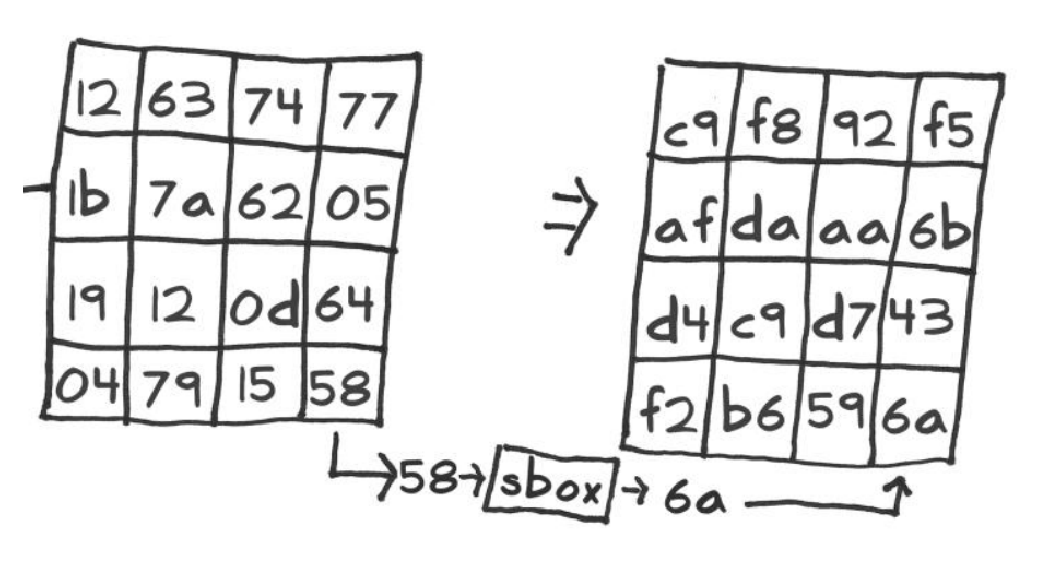
\includegraphics[scale=0.2]{images/Lecture_5/Subbytes.png}
\caption{SubBytes}\label{fig:SubBytes}
\end{figure}

\subsection{ShiftRows}

Then I need to do shift rows. The first row you don't need to do anything, the
other rows you need to shift them, how do you shift with 8-bit microcontroller?
using a temporary value, I read the state into the temporal value and I'm right
it into here. this is also a leaky operation, because I'm leaking all the bytes
in the state, well digging the Hemming Weights of the byte. another way to
implement it, just by imagination, it doesn't change the data so there are
actually operations that don't do shift row.

\begin{figure}[htp]
\centering
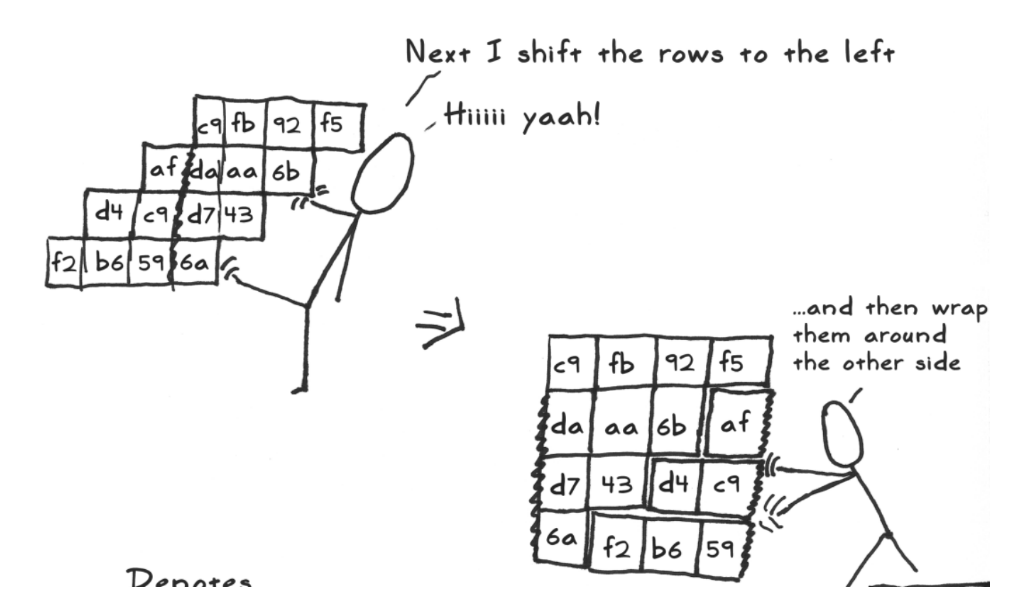
\includegraphics[scale=0.2]{images/Lecture_5/shiftrows.png}
\caption{ShiftRows}\label{fig:ShiftRows}
\end{figure}

\subsection{MixColumns}

Next operation mix columns, is the Matrix a complication, perform over algebra
algorithm, it's takes as input 32 bits columns and his output is 32 bytes value
what are all of the bytes in the output depend of input. How do you do it on a
microcontroller? One of the reasons that rhino run the competition that it was
very efficient way was doing mix column 8-bit microcontroller, using 13
operations which are shifts and exor. This is the most leaky part of AES this
mixed columns.

\begin{figure}[htp]
\centering
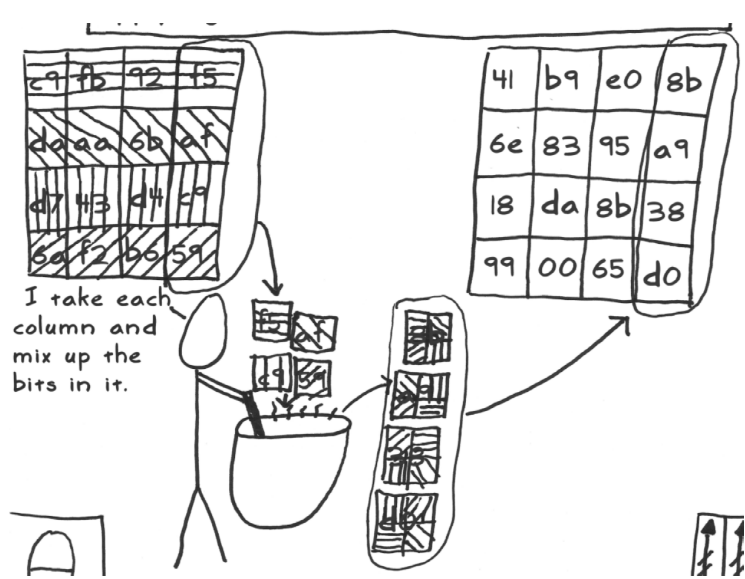
\includegraphics[scale=0.2]{images/Lecture_5/mixcolumns.png}
\caption{MixColumns}\label{fig:MixColumns}
\end{figure}

\subsection{AddRoundKey}

Then do a add round key, just xor, read xor write. This doesn't leak so much
because it is inside the ALU, but the reading and writing is the leaking here.
Each round of AES is 84 leaking actions. You take the key and you use the same
you used to do in creation but you don't have the plane text yet so you use sub
bytes or shift, then you end with the round, and this key expansion is very
sensitive for power analysis, you can really attack as very efficiently. We can
assume that this expansion is very secure.


\begin{figure}[htp]
\centering
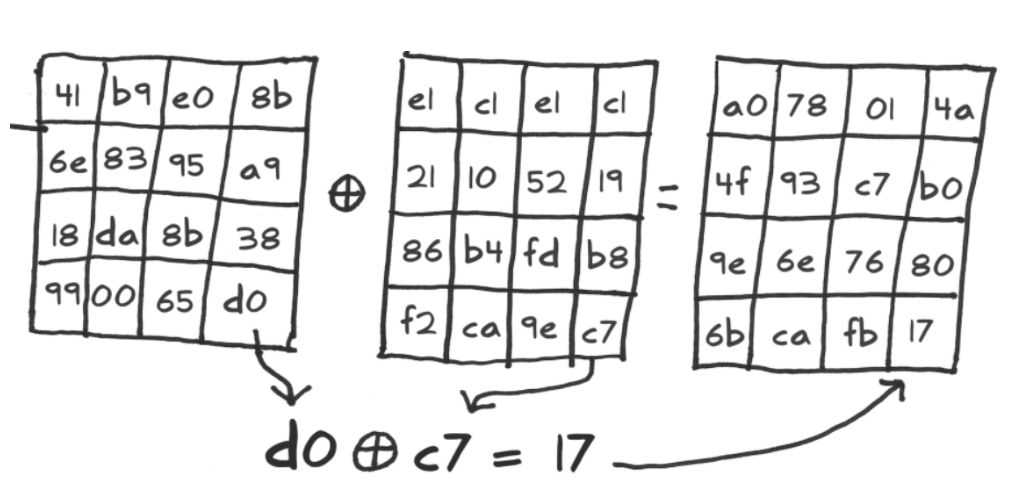
\includegraphics[scale=0.2]{images/Lecture_5/addkey.png}
\caption{AddKey}\label{fig:AddKey}
\end{figure}

\section{AES Power Analysis}
I told you about AES and what is our motivation and what is the structure, and I
want to spend the time that has left to show you a little about internal of AES
and very very very briefly talk about the reaction of doing simple power
analysis of AES. 

\begin{verbatim}
% Make sure the matlab AES scripts are in the path
addpath('matlab_aes_scripts');
%%
% Create two 128-bit plaintexts (exactly 16 byte)
plaintext_1 = uint8('Attack at 12:56!');
plaintext_2 = uint8('Attack at 12:57!');

% how many bits are different between the two?
disp(hamming_weight(bitxor(plaintext_1, plaintext_2)));
%%
% Create a key
key = uint8('1234512345123456');

ENCRYPT = 1;
DECRYPT = 0;
%%
% Encrypt the two plaintexts
ciphertext_1 = aes_crypt_8bit(plaintext_1, key, ENCRYPT); 
ciphertext_2 = aes_crypt_8bit(plaintext_2, key, ENCRYPT);
% even though the plaintexts were very similar...
disp([plaintext_1;plaintext_2]);
% ... the ciphertexts are very different
disp([ciphertext_1;ciphertext_2]);
%%
% how many bits are different between the two?
disp(hamming_weight(bitxor(ciphertext_1, ciphertext_2)));

%%
% Decrypt the two ciphertexts
decrypted_1 =  aes_crypt_8bit(ciphertext_1, key, DECRYPT); 
decrypted_2 =  aes_crypt_8bit(ciphertext_2, key, DECRYPT); 

% Did we get the plaintext again?
disp([plaintext_1;plaintext_2]);
disp([decrypted_1;decrypted_2]);
%%
% Look at the internals of AES now
[ciphertext_1, leak_1] = aes_crypt_8bit_and_leak(plaintext_1, key, ENCRYPT);
[ciphertext_2, leak_2] = aes_crypt_8bit_and_leak(plaintext_2, key, ENCRYPT);

% Show an image showing the two leaks side by size
subplot(1,3,1)
image(squeeze(leak_1));colormap(hsv(256));
subplot(1,3,3)
image(squeeze(leak_2));colormap(hsv(256)); 
figure(gcf)
%%
% Show the difference in the middle
subplot(1,3,2)
image(squeeze(bitxor(leak_1,leak_2)));colormap(hsv(256));
figure(gcf)
%%
% plot the HW of the difference
subplot(1,1,1)
bar(hamming_weight(bitxor(leak_1,leak_2)));
\end{verbatim}

What you see here is Matlab, I wrote this lab environment to do AES
implementations, There is code that dose AES, and there i  code that simulates
the power leakages of AES as it was implemented on 8-bit microcontroller, all of
the operations are 8 bits operations and each time operation happens I'm going
to leak it's Hamming Weight .Let's see what's going on. 

The first thing I'm going to do is to load some libraries and you can find them
in the middle, now going to create 216 bytes plain text. I am going to take
these string, to make it binary string Unit8, and I'm going to measure the
Hamming distance between these two strings. What is the time distance between
these two strings? One, the difference is 6 become 7. 110 - 111.

How do we do it, I have function called bitxor, and this is a vector of size
16,and then waiting Hamming weight. How many possibles Hamming weight are they
for 8 bits value? What can the Hamming weight to be? zero,1,2 … 8.So that
Hamming weight here is going to be one. now I'm going to set up a AES I am going
to choose a key.And now I'm going to encrypt AES, and then I'm going to use my
to plain text and the key. The Hamming distance between the two was one. What
will be the Hamming distance with the cipher text? Will it be one?no! what's
possible values it can be, between 0 to 128, because the output. Would you like
me to be 128? NO, I would like it to be 64. Why do I don't need it to be 100 or
2 or 3. Because that means that I don't have a very important property crypto
assistance in the Avalanche property means that each bit in each bit affect all
of the input. So if I change one bit in the input and I get only one change in
the output it means that I don't have the ability point. But if I change one bit
in the input and I get 100 bit change in the output what it is mean? It's means
that I don't have the average property and just to make things fun I'm flipping
all the bits. What I want the Hamming distance to be is around 64, It's that
exactly half of the bits changing. So you can see I'm doing the Hamming and
measuring and show the ciphertext, at the end I'm doing the Hamming weight.
 
These two strings are very very similar until the end, the 6 and 7 change. But
if you see the ciphertext you can see a lot of difference. And this humming
weight is 52. sometimes he's more sometimes is less than 64 but this is okay.
Now let's decrypt, How do I decrypt? I take my AES 8-bit function and I give it
decrypt. The ciphertext and the key. and see if the plain text into ciphertext
are the same. We can see that there are the same and so far so good. Now I want
to show you the internal structure of AES. to do that I have a function that's
called 8-bit and leak. Let's open the function. Here is the function. Let's go
over the structure

\begin{verbatim}
function [result state rkeys mixcolumn_leak]= 
aes_crypt_8bit_and_leak(input_data, secret_key, encrypt)

% performs AES-128 encryptions or decryptions like an 8-bit uC would do them
% and leaks internal state 
%
% DESCRIPTION:
%
% [result state rkeys mixcolumn_leak] = aes_crypt(input_data, secret_key, encrypt)
%
% This function performs an AES-128 encryption or decryption of the input
% data with the given secret key.
%
% PARAMETERS:
%
% - input_data:
%   A matrix of bytes, where each line consists of a 16 bytes (128 bit)
%   data input value of the AES-128 en/decryption.
% - secret_key:
%   A vector of 16 bytes that represents the secret key.
% - encrypt:
%   Paramter indicating whether an encryption or a decryption is performed
%   (1=encryption, 0=decryption).
%
% RETURNVALUES:
%
% - result:
%   A matrix of bytes of the same size as the byte matrix 'input_data'.
%   Each line of this matrix consists of 16 bytes that represent the
%   128-bit output of an AES-128 en/decryption of the corresponding line of
%   'input_data'.
% - state:
%   A matrix of byte of size |'input_data'| x 41, containins the state
%   progression of the encryption process.  
%   Legend of the state progression:
%   (P= plaintext, C=Ciphertext, K=after AddKey, B=after SubBytes, R=after
%   ShiftRows, M=after MixColumns)
%   P K BRMK BRMK BRMK BRMK BRMK BRMK BRMK BRMK BRMK BRK(=C)
% - mixcolumn_leak:
%   A matrix of size |'input_data'| x 9 x 4 x 9 (for encryption), or
%                    |'input_data'| x 9 x 4 x 18 (for decryption),
%       where mixcolumn_leak(line, subround, col, :) is the list of
%       intermediate valutes generated by the 8-bit MC operation on the
%       [col] columns of line [line] in the input data during
%       subroun [subround]
% EXAMPLE:
%
% result = aes_crypt([1:16; 17:32], 1:16, 1)


% AUTHORS: Stefan Mangard, Mario Kirschbaum, Yossi Oren
%
% CREATION_DATE: 31 July 2001
% LAST_REVISION: 28 October 2008

state = zeros([41 size(input_data)], 'uint8');
rkeys = zeros([10 16], 'uint8');
if (encrypt == 0) % decryption
    mixcolumn_leak = zeros([9 4 size(input_data,1) 18]);
else % encryption
    mixcolumn_leak = zeros([9 4 size(input_data,1) 9]);
end

for round = 1:10
    rkeys(round,:) = aes_round_key(secret_key,round);
end

% expand the keys

if encrypt == 0 %decryption
    state(41,:) = input_data;

    for i=10:-1:1
        if i ~= 10
            input_data = aes_add_round_key( aes_round_key(secret_key,i), input_data);
            state(3 + (i-1)*4 + 2,:) = input_data;

            [input_data leak] = aes_mix_columns_8bit_and_leak(input_data,0);
            mixcolumn_leak(i, :, :, :) = leak;
            state(3 + (i-1)*4 + 1,:) = input_data;
        else
            input_data = aes_add_round_key( aes_round_key(secret_key,i), input_data);
            state(3 + (i-1)*4 + 1,:) = input_data;
        end

        input_data = aes_shift_rows(input_data,0);
        state(3 + (i-1)*4,:) = input_data;

        input_data = uint8(aes_sbox(input_data,0));
        state(3 + (i-1)*4 - 1,:) = input_data;
    end

    input_data = aes_add_round_key(secret_key, input_data);
    state(1,:) = input_data;

else % encryption

    state(1,:) = input_data;
    input_data = aes_add_round_key(secret_key, input_data);
    state(2,:) = input_data;
    
    for i=1:10
        input_data = uint8(aes_sbox(input_data,1));
        state(3 + (i-1)*4,:) = input_data;

        input_data = aes_shift_rows(input_data,1);
        state(3 + (i-1)*4 + 1,:) = input_data;

        if i ~= 10
            [input_data leak] = aes_mix_columns_8bit_and_leak(input_data,1);
            mixcolumn_leak(i, :, :, :) = leak;
            state(3 + (i-1)*4 + 2,:) = input_data;

            input_data = aes_add_round_key( aes_round_key(secret_key,i), input_data);
            state(3 + (i-1)*4 + 3,:) = input_data;
        else
            input_data = aes_add_round_key( aes_round_key(secret_key,i), input_data);
            state(3 + (i-1)*4 + 2,:) = input_data;
        end
    end
            
end

result = input_data;

\end{verbatim}

First of all I expand the key, so I do the AES key expansion and I don't leak
the key expansion. This is the assumption. Let's disregarded that description
for a moment and this is the encryption. First of all I took the state and the
input data in the state, and then I do a add round key, then do SUB bytes, shift
rows, mix column. In the last round I done did you mixed columns, and every time
I do this I don't replace the state and I saved the state. at the end I output
the cipher text, but also the output to the state, so you can see the state is
always changing. Now let's see how does it looks, I'm going to run AES twice,
and then do some little figure.

\begin{figure}[!ht]
\centering
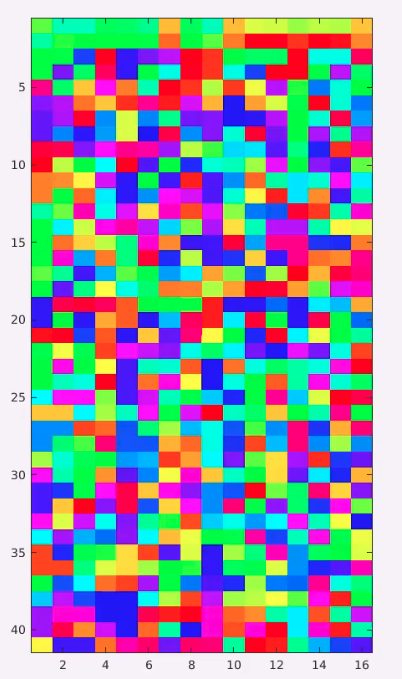
\includegraphics[scale=0.35]{images/Lecture_5/aes_mat_out.png}
\caption{Diagram}\label{fig:Diagram}
\end{figure}

The x-axis is the index of the byte in the state. I read the bytes not as a
matrix I read it as a row. So there are 16 bites in the state. and the y-axis is
the index of the rounds and round 40 is the final round ciphertext. So in
between there is the stages. You can see that in the beginning it is very very
similar.

If you go down it's become much different and in the bottom it's completely
different. This is very easy to analyze. And what we are going to do now show
the difference between state. What do you see in the middle is the Hemming
distance between the right and the left where red is is 0 and blue is 256.

In stage 0 what is the difference between two plain texts? 1 bit, you can see
one beat is changed to O. The first round is a add key, we xor the 15 bytes of
the key who is 16 bytes of the state, the key is the same in both sides, if the
Hamming distance between the two sides was one before I sold the key what is it
going to be after? 1. The differential doesn't change at all, I think a distance
of 1 and Ikes or a constant of both sides and The Outpost is still the same. so
in the first row I can't see differences. look wild sheep will do, one by the
interstate here, one byte is in the same place and one byte There and one byte
here. Now there are 4 bytes different between the states, but this bytes are all
of the column.What is the next operation? mixed columns. See what's mix column
did, mixed this change and now all of the bytes of the states are different.We
can't stop AES after 2 rounds, it still can break with crypto analysis, but you
can see that this is very nice.
 
I want to plug the Hamming weight of the distance, The x-axis here he's there
around, and the y-axis is the Hamming distance between the two stay. you can see
state with the one then one stays one, after sub byte becomes 4, Shift columns
doesn't change the 4, then mix columns make it grow a little bit. And then you
see the distance stays around 64 until the end of the encryption. I want to show
you how do we attack AES using simple power analysis.

There is a lot to talk about in very little time. in very very briefly I will
give you the ideal way did you it and then I'll show you how it's actually done.
I have connected a probe to my device, I have measured the power consumption
overtime. so now I have a vector of size that lets say a hundred thousand, and I
know that AES is there. Now I want to find the key out of my measurements from
my trace.

\begin{figure}[htp]
\centering
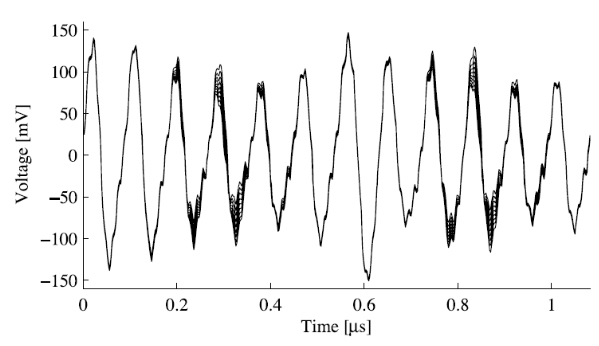
\includegraphics[scale=0.30]{images/Lecture_5/trace1.png}
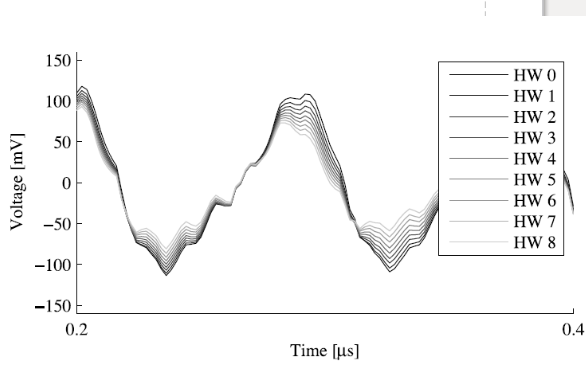
\includegraphics[scale=0.30]{images/Lecture_5/trace2.png}
\caption{Traces}\label{fig:traces}
\end{figure}

I have a trace, which was recorded in the same device we saw here. I have a
vector called 200 of traces of AES encryption, lets plot one of the traces. this
is actually only one of the rounds of AES. Here is a trace. This is very very
clean trace and I would like it to be in my lab.You can see some of them are
high and some of them are low, how do I find the key out of this? let's start
from the beginning then jump to the middle and the end I don't have time to
teach you. the best thing I can hope for is not to get the bytes of the key
because the bytes are not function of the bytes, what is the function of? The
Hamming weight. So the best hope is the get the Hamming weight, so are you home
we will get a vector like the state vector. is this enough to get the key? so
you have to believe me that's yes. how do you do it? You will use algebraic the
solver and you will have to read the paper. if you have the vector off all the
time in Hamming weight you can get the key. But how do I get the vector Hamming
weight from distance? Obviously somewhere in this trace, let's look at very very
leaky operation like sub bytes, or add around key; it read the states you leave
the key and xor them together and then you write the state again. Somewhere in
this vector there is a peak where we know that exactly in this moment there was
a read of the key. The key was read from memory and was travel in the data bus
in this exact peak. And how do I find this particular moment in time I will show
you in the next lecture.

So I need to write a function that gets an input about 20 points and what is its
out puts? the Hamming weight. maybe it will output of Hamming weight. how do I
do it? we need to write a decoder that's as single processing.

Here is a figure showing the move operation they did the same move operation in
the microcontroller over and over again this is the average of thousands of
measurements where are they moving 0 or 1, until moving 255 ff. Can anybody, you
see how Hamming Weight zero have big change, why Hamming weight 0 is more power
consumption of Hamming weight 8? Between moves it settings old ones, so moving
to zero take more effort from changing.
 
Here is like a longer trace, let's assume I hate this data how do I build the
decoder. I want the function that can take an array of values and output Hamming
weight. Let's start simple, what if I had just one point? I have an input and
function that gets one point and give me the Hamming weight of this point. I can
calculate the mean each one, the mean for 0 the mean for 1, for 2. if I get it
right what we will do, so do you like a nearest neighbor. if I know that the
mean of 4 Hamming weight for is 7 and the mean of Hamming weight five is 8 and I
got 7.9, what am I going to chose 4 or 5? 5.nearest neighbor.

This is a nice idea, but I have to give them a little extra dangerous. the
problem is here that's the Hamming weight are not identically distributed. how
many possible values of bytes I get? 256. how many bytes are there with Hamming
weight zero? 1. how many bytes Hamming weight 8? 1. how many Hamming weight 1?
8. Hamming weight of 1 is 8 times more likely than Hamming weight of 0. So why
do we need to do?we need to do Bayes. The idea is are you going to favor the
output more likely. I will found out what are the odds that its five, 6?, 7?
then look on my decoder and then I'm going to look and give a bonus for more
common Hamming weight. The idea is I need to learn How likely bytes based on the
trace decoding and then I'm going to go and look at the distribution of this and
then multiply The probability I got. this is for one point. I calculated the
odds and then I multiply the probability. what if I have more than one point?
watch we actually wants to do here he's actually called multivariate normal
distribution. each one of these points, let's say four points, the dimension,
and I have a like a cloud In this distribution space, how do you do this? that
is the very very fundamental paper called “template power analysis attack” which
explain this.

So if you want to do a simple power analysis on AES the steps you do first of
all you profiled the device, you understand where all this stuff is happening,
you need to build Template that will help you to recognize different Hamming
Weight, then you're play the same place in the trace and you get guesses for
Hamming weight for each States and you hope you get the right guesses, and then
you take this Hamming weight and you take a few equation solver we'll take the
Hamming weight and output the key, or something that we don't know? I don't know
because noise. If we can correlate the Hamming weight to wrong then the equation
solver will fail. what can we do in this case? We try again.

\newpage
\section{Template Attacks} 
\subsection{Introduction}
    Devices performing cryptographic operations can be analyzed by various
    means. Traditional cryptanalysis looks at the relations between input and
    output data and the used keys. However, even if the implemented algorithms
    are secure from a cryptanalysis point of view, side-channel attacks pose a
    serious threat. Sidechannel attacks are a subgroup of implementation
    attacks. Examples thereof are timing attacks, power attacks like DPA or SPA.
    Traditional DPA style attacks assume the following threat model: The secret
    key stored in the device is used to perform some cryptographic operations.
    The attacker monitors these operations using captured side-channel
    information like power consumption or electromagnetic emanation. The attack
    is successful if the used secret key can be reconstructed after a certain
    number of operations.\textbf{If the number of operations is limited by the
    protocol used to initiate} these operations, the attacker has an upper bound
    on the number of operations he can observe. If the operation, which leaks
    usable side-channel information, is executed just once, the threat model is
    different: The attacker has to reconstruct the secret key using a single
    trace of side-channel information. Besides protocol limitations, ephemeral
    keys can be the reason for such a constraint. Techniques like SPA are a
    general way to tackle this problem. These techniques useeasily
    distinguishable features of operations like double and add, or add and
    multiply, to infer key-bits. The majority of the available literature deals
    with these two types of scenarios. \textbf{If the observed signal-to-noise
    ratio is not high enough, or the implementation is done in a way that
    ensures the used operations being independent of the key(i. e. no
    key-dependent jumps), SPA style attacks are not possible anymore.} The
    attacker has to think of other ways to get hold of the secret key: One way
    to do this is to use a similar device and build a model of it. Using this
    model, an attacker might now be able to recover the secret key.
    
\subsection{Algorithm}
    Template attacks are a powerful type of side-channel attack. These attacks
    are a subset of profiling attacks, where an attacker creates a ``profile" of
    a sensitive device and applies this profile to quickly find a victim's
    secret key.
    
    Template attacks require more setup than CPA attacks. To perform a template
    attack, the attacker must have access to another copy of the protected
    device that they can fully control. Then, they must perform a great deal of
    pre-processing to create the template - in practice, this may take dozens of
    thousands of power traces. However, the advantages are that template attacks
    require a very small number of traces from the victim to complete the
    attack. With enough pre-processing, \textbf{the key may be able to be
    recovered from just a single trace} .
    
    
    There are four steps to a template attack:
    \begin{itemize}
      \item Using a copy of the protected device, record a large number of power
      traces using many different inputs (plaintexts and keys). Ensure that
      enough traces are recorded to give us information about each subkey value.
      \item Create a template of the device's operation. This template notes a
      few ``points of interest" in the power traces and a multivariate
      distribution of the power traces at each point.
      \item the victim device, record a small number of power traces. Use
      multiple plaintexts. (We have no control over the secret key, which is
      fixed.)
      \item Apply the template to the attack traces. For each subkey, track
      which value is most likely to be the correct subkey. Continue until the
      key has been recovered.
    \end{itemize}
    
    \subsection{Signals, Noise, and Statistics}
    Before looking at the details of the template attack, it is important to
    understand the statistics concepts that are involved. A template is
    effectively a multivariate distribution that describes several key samples
    in the power traces. This section will describe what a multivariate
    distribution is and how it can be used in this context. Noise
    Distributions\\
    Electrical signals are inherently noisy. Any time we take a voltage
    measurement, we don't expect to see a perfect, constant level. For example,
    if we attached a multi-meter to a 5 V source and took 4 measurements, we
    might expect to see a data set like (4.95, 5.01, 5.06, 4.98). One way of
    modelling this voltage source is: $\mathbf{X} = \mathbf{X} + \mathbf{N}$
    where $\mathbf{X}$ is the noise-free level and $\mathbf{N}$ is the
    additional noise. In our example, $\mathbf{X}$ would be exactly 5 V. Then, N
    is a random variable: every time we take a measurement, we can expect to see
    a different value. Note that $\mathbf{X}$ and $\mathbf{N}$ are bolded to
    show that they are random variables. A simple model for these random
    variables uses a Gaussian distribution (read: a bell curve). The probability
    density function (PDF) of a Gaussian distribution is f(x) = $
    \frac{1}{\sigma \sqrt{2\pi}} e^{-(x - \mu)^2 / 2\sigma^2}$ where
    $\displaystyle \mu$  is the mean and  $ \sigma$ is the standard deviation.
    For instance, our voltage source might have a mean of 5 and a standard
    deviation of 0.5, making the PDF look like:\\
    \begin{minipage}{\linewidth}
    \centering
    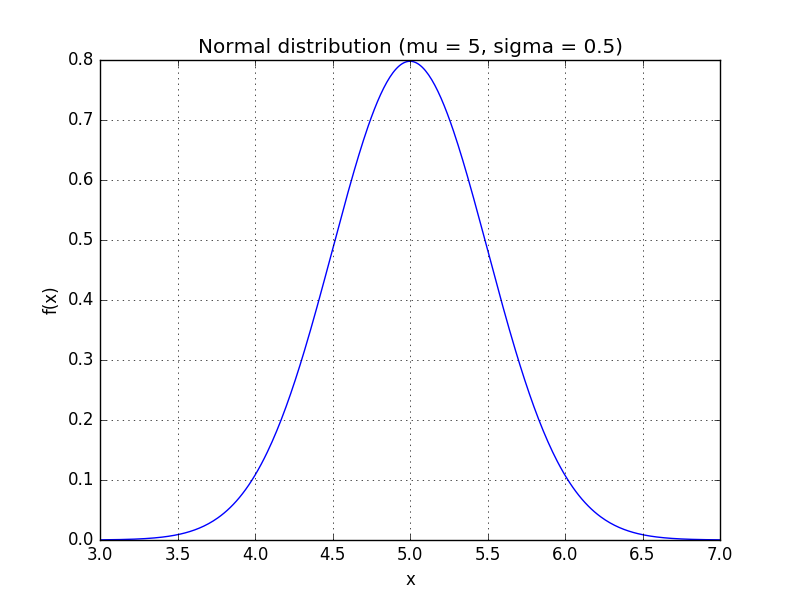
\includegraphics[width=8cm]{images/Lecture_5/Normal-Dist.png}
    \end{minipage}
    We can use the PDF to calculate how likely a certain measurement is. Using
    this distribution, $f(5.1) \approx 0.7821$ $f(7.0) \approx 0.0003$ so we're
    very unlikely to see a reading of 7 V. We'll use this to our advantage in
    this attack: if f(x) is very small for one of our subkey guesses, it's
    probably a wrong guess.\\
    Multivariate Statistics The 1-variable Gaussian distribution works well for
    one measurement. What if we're working with more than one random variable?
    Suppose we're measuring two voltages that have some amount of noise on them.
    We'll call them $\mathbf{X}$ and $\mathbf{Y}$. As a first attempt, we could
    write down a model for $\mathbf{X}$ using a normal distribution and a
    separate model for $\mathbf{Y}$ using a different distribution. However,
    this might not always make sense. If we write two separate distributions,
    what we're saying is that the two variables are independent: when
    $\mathbf{X}$ goes up, there's no guarantee that $\mathbf{Y}$ will follow it.
    Multivariate distributions let us model multiple random variables that may
    or may not be correlated. In a multivariate distribution, instead of writing
    down a single variance $\sigma$, we keep track of a whole matrix of
    covariances. For example, to model three random variables ($\mathbf{X},
    \mathbf{Y}, \mathbf{Z}$), this matrix would be\\
    
    \begin{minipage}{\linewidth}
      \centering
      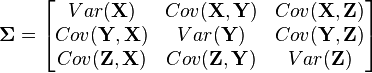
\includegraphics[scale=0.6]{images/Lecture_5/cov.png}
      \end{minipage}\\
      
      
    Also, note that this distribution needs to have a mean for each random
    variable:\\
    
       \begin{minipage}{\linewidth}
      \centering
      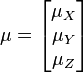
\includegraphics[scale=0.7]{images/Lecture_5/mu.png}
      \end{minipage}\\
      
      
    The PDF of this distribution is more complicated: The equation for k random
    variables is:\\
    
     \begin{minipage}{\linewidth}
      \centering
      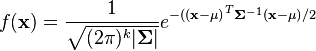
\includegraphics[scale=0.7]{images/Lecture_5/dist.png}
      \end{minipage}

\subsection{Creating the Template}
    A template is a set of probability distributions that describe what the
    power traces look like for many different keys. Effectively, a template
    says: ``If you're going to use key k, your power trace will look like the
    distribution $f_k(\mathbf{x})$"\\
    . We can use this information to find subtle differences between power
    traces and to make very good key guesses for a single power trace.\\
    \\
    \textbf{Number of Traces}\\
    One of the downsides of template attacks is that they require a great number
    of traces to be preprocessed before the attack can begin. This is mainly for
    statistical reasons. In order to come up with a good distribution to model
    the power traces for every key, we need a large number of traces for every
    key. For example, if we're going to attack a single subkey of AES-128, then
    we need to create 256 power consumption models (one for every number from 0
    to 255). In order to get enough data to make good models, we need tens of
    thousands of traces.
    
    Note that we don't have to model every single key. One good alternative is
    to model a sensitive part of the algorithm, like the substitution box in
    AES. We can get away with a much smaller number of traces here; if we make a
    model for every possible Hamming weight, then we would end up with 9 models,
    which is an order of magnitude smaller. However, then we can't recover the
    key from a single attack trace - we need more information to recover the
    secret key.\\
    \\
    \textbf{Points of Interest}\\
    Our goal is to create a multivariate probability describing the power traces
    for every possible key. If we modeled the entire power trace this way (with,
    say, 3000 samples), then we would need a 3000-dimension distribution. This
    is insane, so we'll find an alternative.
    
    Thankfully, not every point on the power trace is important to us. There are
    two main reasons for this:
    \begin{itemize}
      \item We might be taking more than one sample per clock cycle.  There's no
      real reason to use all of these samples - we can get just as much
      information from a single sample at the right time.
      \item Our choice of key doesn't affect the entire power trace. It's likely
      that the subkeys only influence the power consumption at a few critical
      times. If we can pick these important times, then we can ignore most of
      the samples. 
    \end{itemize}
    
    These two points mean that we can usually live with a handful (3-5) of
    points of interest. If we can pick out good points and write down a model
    using these samples, then we can use a 3D or 5D distribution - a great
    improvement over the original 3000D model.
   \subsection{Analyzing the Data}
    Suppose that we've picked I points of interest, which are at samples $s_i (0
    \le i < I)$. Then, our goal is to find a mean and covariance matrix for
    every operation (every choice of subkey or intermediate Hamming weight).
    Let's say that there are K of these operations (maybe 256 subkeys or 9
    possible Hamming weights).
    
    For now, we'll look at a single operation k $(0 \le k < K)$. The steps are:
    \begin{itemize}
      \item Find every power trace t that falls under the category of
      ``operation k". (ex: find every power trace where we used a subkey of
      0x01.) We'll say that there are $T_k$ of these, so $t_{j, s_i}$ means the
      value at trace j and POI i.
      \item Find the average power $\mu_i$ at every point of interest. This
      calculation will look like:
      \begin{figure}[htp]
      \centering
      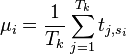
\includegraphics[scale=0.7]{images/Lecture_5/pc1.png}
      \end{figure}
       
      \item Find the variance $v_i$ of the power at each point of interest. One
      way of calculating this is:
      \begin{figure}[htp]
      \centering
      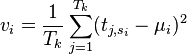
\includegraphics[scale=0.7]{images/Lecture_5/pic2.png}
      \end{figure}
    
      \item Find the covariance $c_{i, i^*}$ between the power at every pair of
      POIs $(i and i^*)$. One way of calculating this is:
      \begin{figure}[htp]
      \centering
      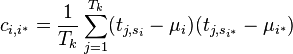
\includegraphics[scale=0.7]{images/Lecture_5/pic3.png}
      \end{figure}
      \item Put together the mean and covariance matrices as:
    
      \begin{minipage}{\linewidth}
      \centering
      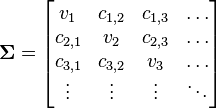
\includegraphics[scale=0.7]{images/Lecture_5/pic5.png}
      \end{minipage}
      \begin{minipage}{\linewidth}
      \centering
      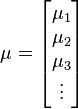
\includegraphics[scale=0.7]{images/Lecture_5/pic4.png}
      \end{minipage}
      
    \end{itemize}
    
    These steps must be done for every operation k. At the end of this
    preprocessing, we'll have K mean and covariance matrices, modelling each of
    the K different operations that the target can do.

    \subsection{Attack Time}
    With a template in hand, we can finish our attack. For the attack, we need a
    smaller number of traces - we'll say that we have A traces. The sample
    values will be labeled $a_{j, s_i} (1 \le j \le A)$. First, let's apply the
    template to a single trace. Our job is to decide how likely all of our key
    guesses are. We need to do the following:
    \begin{itemize}
      \item Put our trace values at the POIs into a vector. This vector will be:
      
       \begin{minipage}{\linewidth}
      \centering
      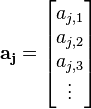
\includegraphics[scale=0.7]{images/Lecture_5/pic6.png}
      \end{minipage}
       
      \item Calculate the PDF for every key guess and save these for later. This
      might look like:
      \begin{minipage}{0cm}
      \centering
      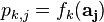
\includegraphics[scale=0.7]{images/Lecture_5/pic7.png}
      \end{minipage}
      \item Repeat these two steps for all of the attack traces
    \end{itemize}
    This process gives us an array of $p_{k, j}$, which says: ``Looking at trace
    j, how likely is it that key k is the correct one?"\\
    \textbf{Combining the Results}\\
    The very last step is to combine our $p_{k, j}$ values to decide which key
    is the best fit. The easiest way to do this is to combine them as:
    
    \begin{figure}[htp]
        \centering
        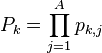
\includegraphics[scale=0.7]{images/Lecture_5/pic8.png}
       \end{figure}
    
    \subsection{practical template attacks}
    In this section we will show a differant ways to select the most important
    point of a power trace, that will lead us to improved computation time and
    make template attack more practical.\\
    \\
    \textbf{sum of difference}
       \begin{itemize}
          \item For every operation k and every sample i, find the average power
          $M_{k, i}$. For instance, if there are $T_k$ traces where we performed
          operation k, then this average is\\
              \begin{minipage}{\linewidth}
              \centering
              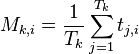
\includegraphics[scale=0.7]{images/Lecture_5/pic9.png}
              \end{minipage}
           
          \item After finding all of the means, calculate all of their absolute
          pairwise differences. Add these up. This will give one ``trace" which
          has peaks where the samples are usually different. The calculation
          looks like\\
          \\
              \begin{minipage}{\linewidth}
              \centering
              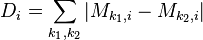
\includegraphics[scale=0.7]{images/Lecture_5/pic10.png}
              \end{minipage}
       \end{itemize}
        An example of this sum of differences is:\\
              \begin{minipage}{\linewidth}
              \centering
              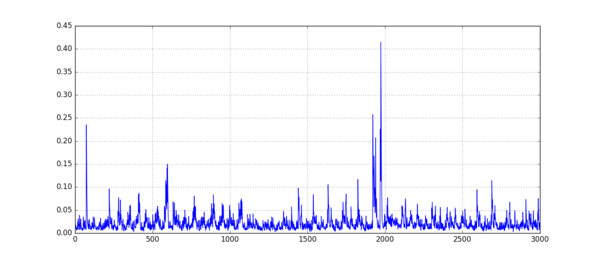
\includegraphics[scale=0.7]{images/Lecture_5/pic11.png}
              \end{minipage}
        \\

\textbf{Preprocessing}\\
    In practical side-channel analysis, the raw input data is often
    preprocessed. Sometimes this is just due to simplicity or efficiency
    reasons, e. g. summarizing sampled points. There are however cases where the
    preprocessing step heavily affects the results. Even if no thinkable
    transformation can add additional information to a signal, information
    extraction procedures do improve. The template attack under consideration is
    such a case and a lucrative preprocessing transformation is described
    subsequently. It turns out that the transformation of the input traces from
    the time domain into the frequency domain is such a lucrative
    transformation. In our practical work, an FFT algorithm was used to
    accomplish this transformation (a fast algorithm to calculate the discrete
    Fourier transform, for background information refer to [BP85]). In order to
    show the impact of this preprocessing step a number of experiments were
    carried out. First some characteristic differences between time domain
    analysis and frequency domain analysis are illustrated. Afterwards, to
    highlight the influence of the number of selected points on the
    classification performance in the frequency domain, a number of experiments
    were carried out. After preprocessing, the resulting traces can be used to
    perform a template attack in exact the same way as without preprocessing.
    There is however a difference in the number of points to consider. Figure 6
    shows the classifications results as a function of the number of selected
    points after preprocessing. The considered numbers of points are ranging
    between 1 and 40. Additionally three different minimum distances where
    chosen. Results show that much less points are sufficient in comparison to a
    template attack without the preprocessing step. At the price of performing
    an FFT on every input trace (those used to build up the templates as well as
    those to classify) we get a major advantage\\


\textbf{Amplified Template Attack}

    Even if the aim of a template attack is to recover the secret key using a
    single trace, in many real world settings implementations allow for several
    iterations of the same operation with the same secret key. The application
    of template attacks is not restricted to stream ciphers like RC4 and can be
    applied to block ciphers as well. Since every symmetric cipher contains some
    sort of key scheduling mechanism which processes the secret key, this
    generalization is possible. Smartcards often use block ciphers for
    encryption or authentication, hence let us consider the following example: A
    malicious petrol station tenant, named Eve, is using a modified smartcard
    based payment terminal. Everytime a customer uses this terminal, Eve
    captures one trace of side-channel information. This single trace could
    already be used by Eve to carry out a template attack. However, some
    customers are coming again and Eve gets hold of another trace. The template
    attack can easily be extended to take advantage of such situations, e.g. by
    adding up noise-probabilities p(Ni) of every captured trace and applying the
    maximum-likelihood approach on these sums. As a consequence, the power of
    the attacker is amplified. Using this approach, if n is the number of
    iterations, the error probability of template classification is reduced by
    the factor √n. 
